
\subsection*{3.3 Longitude and Latitude Problems, Bearings}
Longitude and latitude are used to specify the position of points on the Earth's surface. Bearings and directions play a crucial role in navigation and solving geographical problems.

\textbf{Key Concepts:}
\begin{itemize}
	\item \textbf{Bearing of an Angle:} Bearings are used to describe the direction of one point relative to another. Bearings are measured clockwise from the north direction and are usually expressed in three digits. For example, $045^\circ$ represents a bearing of $45^\circ$ from north.
	\begin{center}
		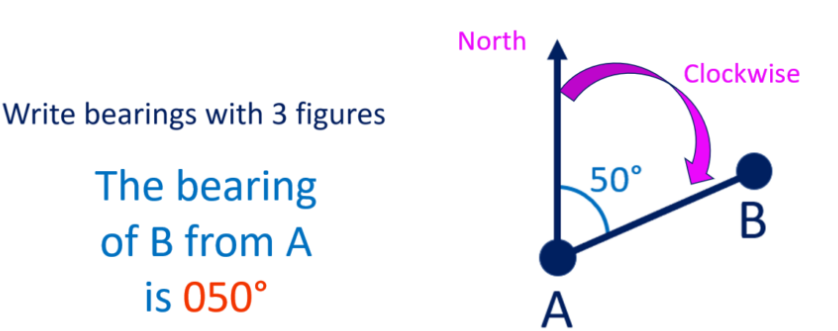
\includegraphics[width=0.6\textwidth]{3.7.png}
	\end{center}
	\item \textbf{Main Directions:} The primary compass directions are:
	\begin{itemize}
		\item \textbf{North (N):} $0^\circ$ or $360^\circ$
		\item \textbf{East (E):} $90^\circ$
		\item \textbf{South (S):} $180^\circ$
		\item \textbf{West (W):} $270^\circ$
	\end{itemize}
\end{itemize}

\textbf{Examples:}

\begin{flushleft}
	\textbf{Example 1: A ship travels on a bearing of $120^\circ$. What direction is the ship moving?}
	
	\vspace{0.5cm}
	\textbf{Solution:}
	\vspace{0.5cm}
	
	A bearing of $120^\circ$ is measured clockwise from north. This places the direction in the southeast quadrant. Therefore, the ship is moving southeast.
\end{flushleft}

\begin{flushleft}
	\textbf{Example 2: Find the bearing from Point A to Point B if A is due west of B.}
	
	\vspace{0.5cm}
	\textbf{Solution:}
	\vspace{0.5cm}
	
	If A is due west of B, the bearing from A to B is measured clockwise from north:
	\[
	\text{Bearing} = 270^\circ.
	\]
	
	Therefore, the bearing is $270^\circ$.
\end{flushleft}

\begin{flushleft}
	\textbf{Example 3: John was facing $S35^\circ E$. If he turned $90^\circ$ in the anticlockwise direction, find his new direction.}
	
	\vspace{0.5cm}
	\textbf{Solution:}
	\vspace{0.5cm}
	
	Step 1: Convert $S35^\circ E$ to a bearing:
	\[
	\text{Bearing} = 180^\circ - 35^\circ = 145^\circ.
	\]
	
	Step 2: Subtract $90^\circ$ for the anticlockwise turn:
	\[
	145^\circ - 90^\circ = 55^\circ.
	\]
	
	Step 3: Convert the bearing back to a compass direction:
	\[
	55^\circ \text{ is measured as } N55^\circ E.
	\]
	
	Therefore, John's new direction is $N55^\circ E$ (bearing of $55^\circ$).
\end{flushleft}


\begin{flushleft}
	\textbf{Example 3:} The bearing of $Q$ from $P$ is $015^\circ$ and the bearing of $P$ from $R$ is $015^\circ$. If $Q$ and $R$ are $24$ km and $32$ km respectively from $P$:
	
	\begin{enumerate}
		\item[(i)] Represent this information in a diagram.
		\item[(ii)] Calculate the distance between $Q$ and $R$, correct to two decimal places.
		\item[(iii)] Find the bearing of $R$ from $Q$, correct to the nearest degree.
	\end{enumerate}
	
	\vspace{0.5cm}
	\begin{center}
		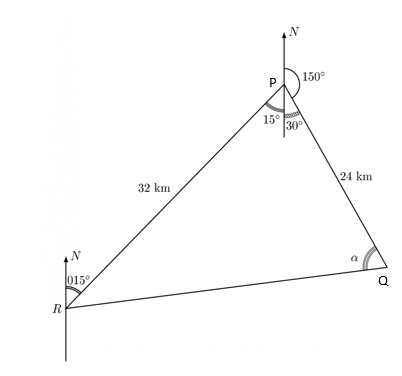
\includegraphics[width=0.6\textwidth]{3.21.png}
	\end{center}
	
	\textbf{Solution:}
	\vspace{0.5cm}
	
	Step 1: Represent the given bearings in a diagram. Since both bearings are measured from the north, we construct a diagram accordingly.
	
	Step 2: Use the cosine rule to find the distance between $Q$ and $R$. The angle between $PQ$ and $PR$ is:
	\[
	\theta = (15^\circ + 35^\circ) = 145^\circ.
	\]
	Using the cosine rule:
	
	\[
	|QR|^2 = 32^2 + 24^2 - 2 \times 32 \times 24 \times \cos 45^\circ
	\]
	
	\[
	|QR|^2 = 1024 + 576 - 1536 \cos 45^\circ
	\]
	
	\[
	= 1600 - 1086.1056
	\]
	
	\[
	|QR|^2 = 513.8944
	\]
	
	\[
	|QR| = \sqrt{513.8944} = 22.669 \text{ km}
	\]
	
	\[
	\approx 22.67 \text{ km to 2 dp} 
	\]
	
	
	
	Step 3: Find the angle $\angle$ PQR using the sine rule:
	\[
	\frac{32}{\sin \angle PQR} = \frac{22.67}{\sin 45^\circ}
	\]
	
	\[
	\sin \angle PQR = \frac{32 \times \sin 45^\circ}{22.67}
	\]
	
	\[
	= 0.9981
	\]
	
	\[
	\angle PQR = \sin^{-1} (0.9981) = 86.4787^\circ
	\]
	
	
	
	Step 4: Calculate the bearing of $R$ from $Q$:
	\\
	\begin{center}
		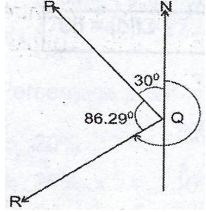
\includegraphics[width=0.6\textwidth]{3.11.png}
	\end{center}
	The bearing of R from Q is given by the reflex angle NQR. Thus,
	
	\[
	\text{Reflex } \angle NQR = 360^\circ - (86.47^\circ + 30^\circ)
	\]
	
	\[
	= 360^\circ - 116.47^\circ
	\]
	
	\[
	= 243.53^\circ
	\]
	
	Hence, the bearing of R from Q:
	
	\[
	\approx 244^\circ \quad (\text{to the nearest degree})
	\]
	
	
\end{flushleft}


